\documentclass[10pt,ignorenonframetext,,aspectratio=149]{beamer}
\usefonttheme{serif} % use mainfont rather than sansfont for slide text
\setbeamertemplate{caption}[numbered]
\setbeamertemplate{caption label separator}{: }
\setbeamercolor{caption name}{fg=normal text.fg}
\usepackage{lmodern}
\usepackage{amssymb,amsmath}
\usepackage{ifxetex,ifluatex}
\usepackage{fixltx2e} % provides \textsubscript
\ifnum 0\ifxetex 1\fi\ifluatex 1\fi=0 % if pdftex
  \usepackage[T1]{fontenc}
  \usepackage[utf8]{inputenc}
\else % if luatex or xelatex
  \ifxetex
    \usepackage{mathspec}
  \else
    \usepackage{fontspec}
  \fi
  \defaultfontfeatures{Ligatures=TeX,Scale=MatchLowercase}
  \newcommand{\euro}{€}
    \setmainfont[]{Open Sans}
\fi
% use upquote if available, for straight quotes in verbatim environments
\IfFileExists{upquote.sty}{\usepackage{upquote}}{}
% use microtype if available
\IfFileExists{microtype.sty}{%
\usepackage{microtype}
\UseMicrotypeSet[protrusion]{basicmath} % disable protrusion for tt fonts
}{}
\usepackage{color}
\usepackage{fancyvrb}
\newcommand{\VerbBar}{|}
\newcommand{\VERB}{\Verb[commandchars=\\\{\}]}
\DefineVerbatimEnvironment{Highlighting}{Verbatim}{commandchars=\\\{\}}
% Add ',fontsize=\small' for more characters per line
\usepackage{framed}
\definecolor{shadecolor}{RGB}{248,248,248}
\newenvironment{Shaded}{\begin{snugshade}}{\end{snugshade}}
\newcommand{\AlertTok}[1]{\textcolor[rgb]{0.94,0.16,0.16}{#1}}
\newcommand{\AnnotationTok}[1]{\textcolor[rgb]{0.56,0.35,0.01}{\textbf{\textit{#1}}}}
\newcommand{\AttributeTok}[1]{\textcolor[rgb]{0.77,0.63,0.00}{#1}}
\newcommand{\BaseNTok}[1]{\textcolor[rgb]{0.00,0.00,0.81}{#1}}
\newcommand{\BuiltInTok}[1]{#1}
\newcommand{\CharTok}[1]{\textcolor[rgb]{0.31,0.60,0.02}{#1}}
\newcommand{\CommentTok}[1]{\textcolor[rgb]{0.56,0.35,0.01}{\textit{#1}}}
\newcommand{\CommentVarTok}[1]{\textcolor[rgb]{0.56,0.35,0.01}{\textbf{\textit{#1}}}}
\newcommand{\ConstantTok}[1]{\textcolor[rgb]{0.00,0.00,0.00}{#1}}
\newcommand{\ControlFlowTok}[1]{\textcolor[rgb]{0.13,0.29,0.53}{\textbf{#1}}}
\newcommand{\DataTypeTok}[1]{\textcolor[rgb]{0.13,0.29,0.53}{#1}}
\newcommand{\DecValTok}[1]{\textcolor[rgb]{0.00,0.00,0.81}{#1}}
\newcommand{\DocumentationTok}[1]{\textcolor[rgb]{0.56,0.35,0.01}{\textbf{\textit{#1}}}}
\newcommand{\ErrorTok}[1]{\textcolor[rgb]{0.64,0.00,0.00}{\textbf{#1}}}
\newcommand{\ExtensionTok}[1]{#1}
\newcommand{\FloatTok}[1]{\textcolor[rgb]{0.00,0.00,0.81}{#1}}
\newcommand{\FunctionTok}[1]{\textcolor[rgb]{0.00,0.00,0.00}{#1}}
\newcommand{\ImportTok}[1]{#1}
\newcommand{\InformationTok}[1]{\textcolor[rgb]{0.56,0.35,0.01}{\textbf{\textit{#1}}}}
\newcommand{\KeywordTok}[1]{\textcolor[rgb]{0.13,0.29,0.53}{\textbf{#1}}}
\newcommand{\NormalTok}[1]{#1}
\newcommand{\OperatorTok}[1]{\textcolor[rgb]{0.81,0.36,0.00}{\textbf{#1}}}
\newcommand{\OtherTok}[1]{\textcolor[rgb]{0.56,0.35,0.01}{#1}}
\newcommand{\PreprocessorTok}[1]{\textcolor[rgb]{0.56,0.35,0.01}{\textit{#1}}}
\newcommand{\RegionMarkerTok}[1]{#1}
\newcommand{\SpecialCharTok}[1]{\textcolor[rgb]{0.00,0.00,0.00}{#1}}
\newcommand{\SpecialStringTok}[1]{\textcolor[rgb]{0.31,0.60,0.02}{#1}}
\newcommand{\StringTok}[1]{\textcolor[rgb]{0.31,0.60,0.02}{#1}}
\newcommand{\VariableTok}[1]{\textcolor[rgb]{0.00,0.00,0.00}{#1}}
\newcommand{\VerbatimStringTok}[1]{\textcolor[rgb]{0.31,0.60,0.02}{#1}}
\newcommand{\WarningTok}[1]{\textcolor[rgb]{0.56,0.35,0.01}{\textbf{\textit{#1}}}}
\usepackage{graphicx,grffile}
\makeatletter
\def\maxwidth{\ifdim\Gin@nat@width>\linewidth\linewidth\else\Gin@nat@width\fi}
\def\maxheight{\ifdim\Gin@nat@height>\textheight0.8\textheight\else\Gin@nat@height\fi}
\makeatother
% Scale images if necessary, so that they will not overflow the page
% margins by default, and it is still possible to overwrite the defaults
% using explicit options in \includegraphics[width, height, ...]{}
\setkeys{Gin}{width=\maxwidth,height=\maxheight,keepaspectratio}

% Comment these out if you don't want a slide with just the
% part/section/subsection/subsubsection title:
\AtBeginPart{
  \let\insertpartnumber\relax
  \let\partname\relax
  \frame{\partpage}
}
\AtBeginSection{
  \let\insertsectionnumber\relax
  \let\sectionname\relax
  \frame{\sectionpage}
}
\AtBeginSubsection{
  \let\insertsubsectionnumber\relax
  \let\subsectionname\relax
  \frame{\subsectionpage}
}

\setlength{\emergencystretch}{3em}  % prevent overfull lines
\providecommand{\tightlist}{%
  \setlength{\itemsep}{0pt}\setlength{\parskip}{0pt}}
\setcounter{secnumdepth}{0}

\title{Pengenalan data sains dasar dan R}
\subtitle{(Pelatihan data sains menggunakan R dan Gephi)}
\author{Ujang Fahmi}
\date{}

%% Here's everything I added.
%%--------------------------

\usepackage{graphicx}
\usepackage{rotating}
%\setbeamertemplate{caption}[numbered]
\usepackage{hyperref}
\usepackage{caption}
\usepackage[normalem]{ulem}
%\mode<presentation>
\usepackage{wasysym}
%\usepackage{amsmath}


% Get rid of navigation symbols.
%-------------------------------
\setbeamertemplate{navigation symbols}{}

% Optional institute tags and titlegraphic.
% Do feel free to change the titlegraphic if you don't want it as a Markdown field.
%----------------------------------------------------------------------------------
\institute{Pelajaran ke-1}

% \titlegraphic{\includegraphics[width=0.3\paperwidth]{\string~/Dropbox/teaching/clemson-academic.png}} % <-- if you want to know what this looks like without it as a Markdown field. 
% -----------------------------------------------------------------------------------------------------
\titlegraphic{
\includegraphics[width=0.3\paperwidth]{styles/sadasa.png}}

% Some additional title page adjustments.
%----------------------------------------
\setbeamertemplate{title page}[empty]
%\date{}
\setbeamerfont{subtitle}{size=\small}

\setbeamercovered{transparent}

% Some optional colors. Change or add as you see fit.
%---------------------------------------------------
\definecolor{clemsonpurple}{HTML}{522D80}
 \definecolor{clemsonorange}{HTML}{F66733}
\definecolor{uiucblue}{HTML}{003C7D}
\definecolor{uiucorange}{HTML}{F47F24}


% Some optional color adjustments to Beamer. Change as you see fit.
%------------------------------------------------------------------
\setbeamercolor{frametitle}{fg=clemsonpurple,bg=white}
\setbeamercolor{title}{fg=clemsonpurple,bg=white}
\setbeamercolor{local structure}{fg=clemsonpurple}
\setbeamercolor{section in toc}{fg=clemsonpurple,bg=white}
% \setbeamercolor{subsection in toc}{fg=clemsonorange,bg=white}
\setbeamercolor{footline}{fg=clemsonpurple!50, bg=white}
\setbeamercolor{block title}{fg=clemsonorange,bg=white}


\let\Tiny=\tiny


% Sections and subsections should not get their own damn slide.
%--------------------------------------------------------------
\AtBeginPart{}
\AtBeginSection{}
\AtBeginSubsection{}
\AtBeginSubsubsection{}

% Suppress some of Markdown's weird default vertical spacing.
%------------------------------------------------------------
\setlength{\emergencystretch}{0em}  % prevent overfull lines
\setlength{\parskip}{0pt}


% Allow for those simple two-tone footlines I like. 
% Edit the colors as you see fit.
%--------------------------------------------------
\defbeamertemplate*{footline}{my footline}{%
    \ifnum\insertpagenumber=1
    \hbox{%
        \begin{beamercolorbox}[wd=\paperwidth,ht=.8ex,dp=1ex,center]{}%
      % empty environment to raise height
        \end{beamercolorbox}%
    }%
    \vskip0pt%
    \else%
        \Tiny{%
            \hfill%
		\vspace*{1pt}%
            \insertframenumber/\inserttotalframenumber \hspace*{0.1cm}%
            \newline%
            \color{clemsonpurple}{\rule{\paperwidth}{0.4mm}}\newline%
            \color{clemsonorange}{\rule{\paperwidth}{.4mm}}%
        }%
    \fi%
}

% Various cosmetic things, though I must confess I forget what exactly these do and why I included them.
%-------------------------------------------------------------------------------------------------------
\setbeamercolor{structure}{fg=blue}
\setbeamercolor{local structure}{parent=structure}
\setbeamercolor{item projected}{parent=item,use=item,fg=clemsonpurple,bg=white}
\setbeamercolor{enumerate item}{parent=item}

% Adjust some item elements. More cosmetic things.
%-------------------------------------------------
\setbeamertemplate{itemize item}{\color{clemsonpurple}$\bullet$}
\setbeamertemplate{itemize subitem}{\color{clemsonpurple}\scriptsize{$\bullet$}}
\setbeamertemplate{itemize/enumerate body end}{\vspace{.6\baselineskip}} % So I'm less inclined to use \medskip and \bigskip in Markdown.

% Automatically center images
% ---------------------------
% Note: this is for ![](image.png) images
% Use "fig.align = "center" for R chunks

\usepackage{etoolbox}

\AtBeginDocument{%
  \letcs\oig{@orig\string\includegraphics}%
  \renewcommand<>\includegraphics[2][]{%
    \only#3{%
      {\centering\oig[{#1}]{#2}\par}%
    }%
  }%
}

% I think I've moved to xelatex now. Here's some stuff for that.
% --------------------------------------------------------------
% I could customize/generalize this more but the truth is it works for my circumstances.

\ifxetex
\setbeamerfont{title}{family=\fontspec{Titillium Web}}
\setbeamerfont{frametitle}{family=\fontspec{Titillium Web}}
\usepackage[font=small,skip=0pt]{caption}
 \else
 \fi

% Okay, and begin the actual document...

\begin{document}
\frame{\titlepage}

\begin{frame}
Salam kenal dan selamat datang.

Semoga kita semua bisa saling berbagi pengalaman dan pengetahuan. Saya
adalah Ujang Fahmi, Co-founder dan mentor Sadasa Academy.

\vspace{0.1in}

Jika anda berada dan sedang membaca tutorial ini, maka kemungkinan anda
adalah orang yang sedang ingin belajar data sains, atau mungkin
ditugaskan untuk mempelajari R oleh institusi atau organisasi anda. Sama
seperti saya dulu, dimana tanpa latar belakang enginering saya
didiharuskan untuk belajar R, demi menyelesaikan tugas akhir dan
akhirnya jadilah seperti saya sekarang ini.

\vspace{0.1in}

Satu hal yang pasti, ini adalah langkah pertama dari banyak langkah yang
harus dilalui, entah melalui lembaga resmi atau belajar secara mandiri.
Jadi selamat belajar!!!

\vspace{0.1in}

Ujang Fahmi,

Yogyakarta, 2021-09-17
\end{frame}

\hypertarget{pengenalan-data-sains}{%
\section{Pengenalan Data Sains}\label{pengenalan-data-sains}}

\begin{frame}{Apa itu data sains?}
\protect\hypertarget{apa-itu-data-sains}{}
\begin{columns}[T]
\begin{column}{0.5\textwidth}
Data Sains merupakan sebuah bidang inter atau bahkan multidisiplin yang
menggunakan metode-metode saintifik, proses, algoritma, dan sistem untuk
mengekstrak pengetahuan dari data yang terstruktur, tidak terstruktur
dan bercabang.

\begin{itemize}
\tightlist
\item
  Memiliki keterampilan koding
\item
  Mengetahui dan menguasai matematika dan statistik
\item
  Memiliki domain knowledge spesifik yang kuat
\end{itemize}
\end{column}

\begin{column}{0.5\textwidth}
Keterampilan data seorang data saintis
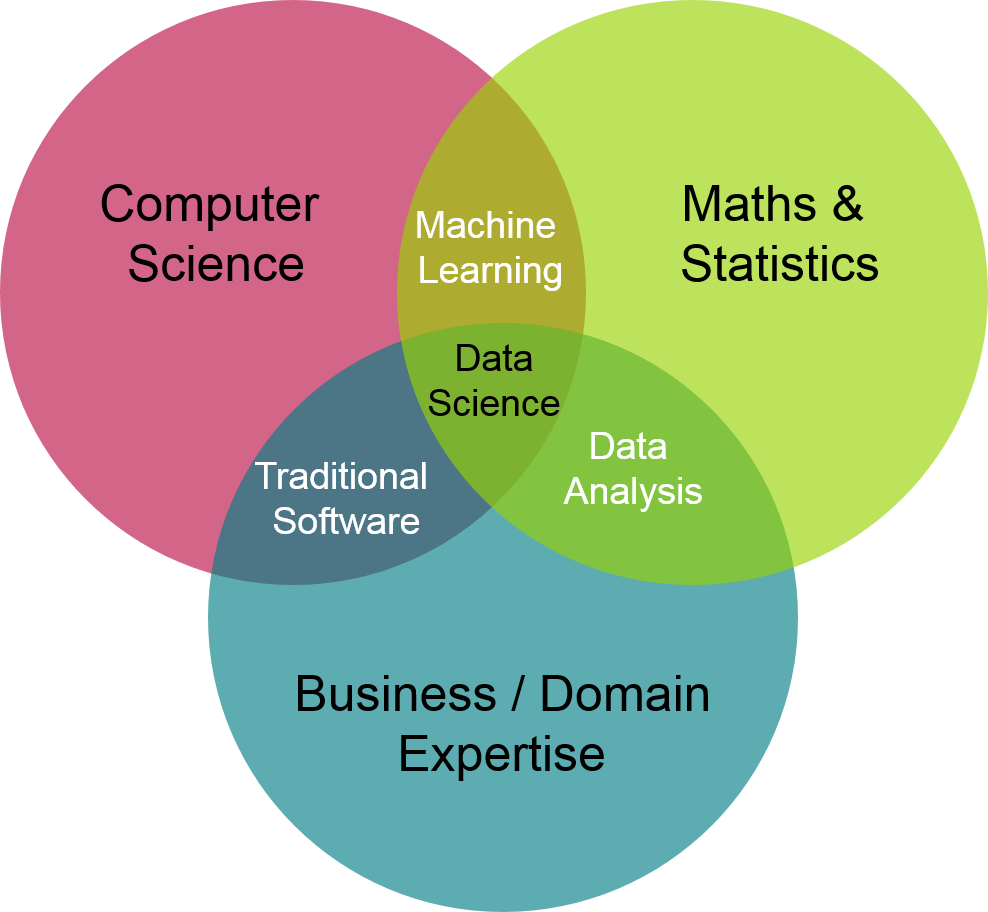
\includegraphics{images/introtods1.png}
\end{column}
\end{columns}
\end{frame}

\begin{frame}{Sosial data sains?}
\protect\hypertarget{sosial-data-sains}{}
\begin{columns}[T]
\begin{column}{0.4\textwidth}
Social data science is a new discipline combining the social sciences
and computer science in which the analysis of big data is linked to
social scientific theory and analysis.
\end{column}

\begin{column}{0.6\textwidth}
\href{https://www.ox.ac.uk/admissions/graduate/courses/msc-social-data-science}{https://www.ox.ac.uk/}

\begin{figure}
\centering

\includegraphics{images/introtods2.png}
\caption{Program Social Data Science di Oxford}
\end{figure}
\end{column}
\end{columns}
\end{frame}

\begin{frame}{Alat-alat yang biasa digunakan}
\protect\hypertarget{alat-alat-yang-biasa-digunakan}{}
\begin{columns}[T]
\begin{column}{0.5\textwidth}
\begin{block}{Umum}
\protect\hypertarget{umum}{}
Bahasa pemerograman yang biasa digunakan untuk mengolah data

\begin{itemize}
\tightlist
\item
  R - \href{https://www.r-project.org/}{statistical programming
  language}
\item
  Python - \href{https://www.python.org/}{general programming language}
\item
  Julia - \href{https://julialang.org/}{programming language untuk big
  data}
\end{itemize}
\end{block}
\end{column}

\begin{column}{0.5\textwidth}
\begin{block}{Spesifik}
\protect\hypertarget{spesifik}{}
Perangkat lunak yang biasa digunakan untuk mengolah data dengan tujuan
spesifik

\begin{itemize}
\tightlist
\item
  Gephi - \href{https://gephi.org/}{Network Analysis}
\item
  Nodexl - \href{https://nodexl.com/}{Network Analysis}
\item
  Orange - \href{https://orangedatamining.com/}{Data Mining}
\end{itemize}
\end{block}
\end{column}
\end{columns}
\end{frame}

\begin{frame}{Harus menggunakan yang mana?}
\protect\hypertarget{harus-menggunakan-yang-mana}{}
\begin{itemize}
\tightlist
\item
  Pilih yang sudah banyak digunakan oleh orang lain
\item
  Pilih yang memiliki komunitas yang kuat baik di dunia maupun di negara
  kita
\item
  Pilih yang sesuai dengan kebutuhan
\item
  Pelajari semuanya, pilih salah satu untuk dikuasai
\end{itemize}
\end{frame}

\hypertarget{r-dan-rstudio}{%
\section{R dan Rstudio}\label{r-dan-rstudio}}

\begin{frame}[fragile]{Kenapa menggunakan R dan Rstudio}
\protect\hypertarget{kenapa-menggunakan-r-dan-rstudio}{}
\begin{columns}[T]
\begin{column}{0.5\textwidth}
\begin{itemize}
\tightlist
\item
  \texttt{R} adalah bahasa pemerogramannya
\item
  \texttt{R\ Studio} adalah perangkat lunak yang menjadi interpreter
  \texttt{R}
\item
  \texttt{R\ Studio} adalah merupakan salah satu lembaga yang
  berkontribusi besar dalam perkembangan \texttt{R}
\item
  Apakah R bisa dijalankan di IDE lain? Ya, bisa. Misalnya di
  \texttt{VsCode}
\end{itemize}
\end{column}

\begin{column}{0.5\textwidth}
\begin{figure}
\centering
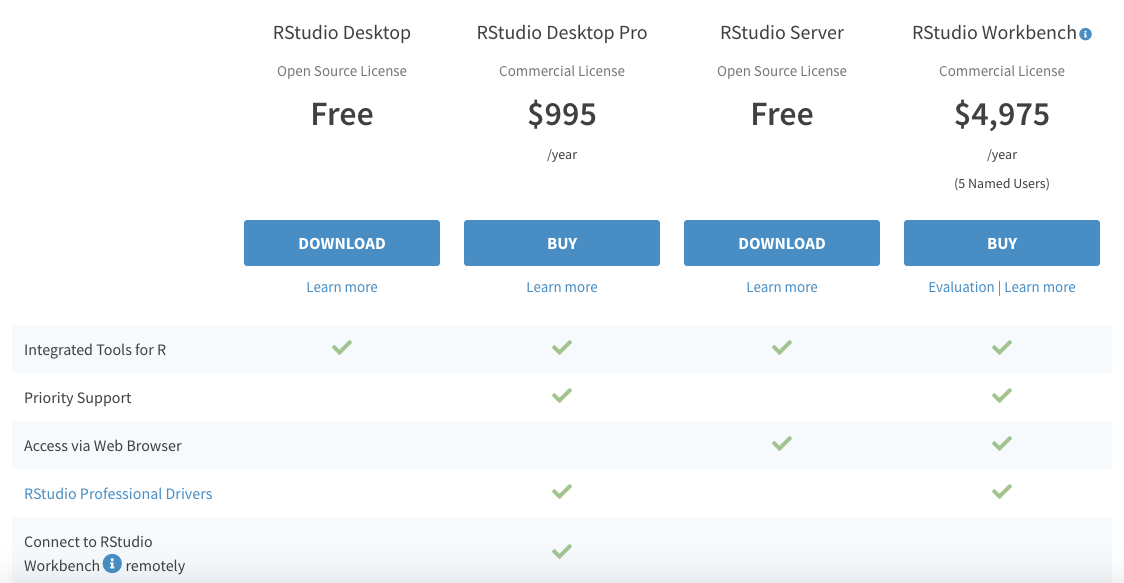
\includegraphics{images/introtods3.png}
\caption{Pilihan R Studio yang bisa didapat}
\end{figure}
\end{column}
\end{columns}
\end{frame}

\begin{frame}{Mendapatakan R dan Rstudio}
\protect\hypertarget{mendapatakan-r-dan-rstudio}{}
\begin{columns}[T]
\begin{column}{0.5\textwidth}
\begin{itemize}
\tightlist
\item
  R bisa didapatkan di \url{https://www.r-project.org/}
\item
  R Studio bisa didapatkan di
  \url{https://www.rstudio.com/products/rstudio/download/}
\end{itemize}
\end{column}

\begin{column}{0.5\textwidth}
\begin{figure}
\centering

\includegraphics{images/introtods4.png}
\caption{Pilihan R Studio yang bisa didapat}
\end{figure}
\end{column}
\end{columns}
\end{frame}

\begin{frame}{Bisa apa saja dengan R dan Rstudio}
\protect\hypertarget{bisa-apa-saja-dengan-r-dan-rstudio}{}
Saat ini dengan menggunakan R dan Rstudio kita hampir bisa melakukan
semua kegiatan yang berkaitan dengan pengolahan data, misalnya:

\begin{itemize}
\tightlist
\item
  Mendapatkan data
\item
  Melakukan manipulasi atau pra-pemerosesan
\item
  Membuat analisis dengan statistik, Macine Learning dan Deep Learning
\item
  Membuat laporan hasil pengolahan data
\item
  Membuat dashboard hasil pengolahan data
\end{itemize}
\end{frame}

\begin{frame}{Gallery Shiny Dashboard}
\protect\hypertarget{gallery-shiny-dashboard}{}
\begin{figure}
\centering
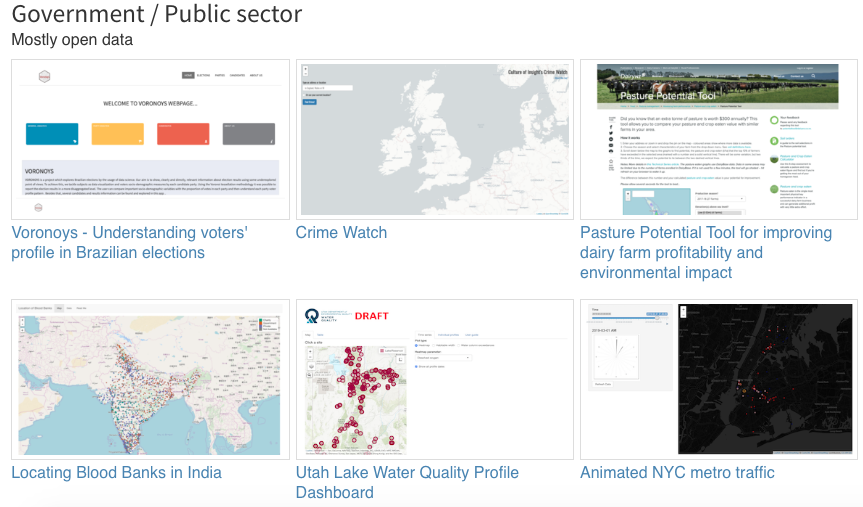
\includegraphics{images/introtods5.png}
\caption{Shiny Dashboard salah satu output R}
\end{figure}
\end{frame}

\hypertarget{menggunakan-r-dan-rstudio}{%
\section{Menggunakan R dan Rstudio}\label{menggunakan-r-dan-rstudio}}

\begin{frame}{Menggunakan R dan Rstudio}
\begin{figure}
\centering
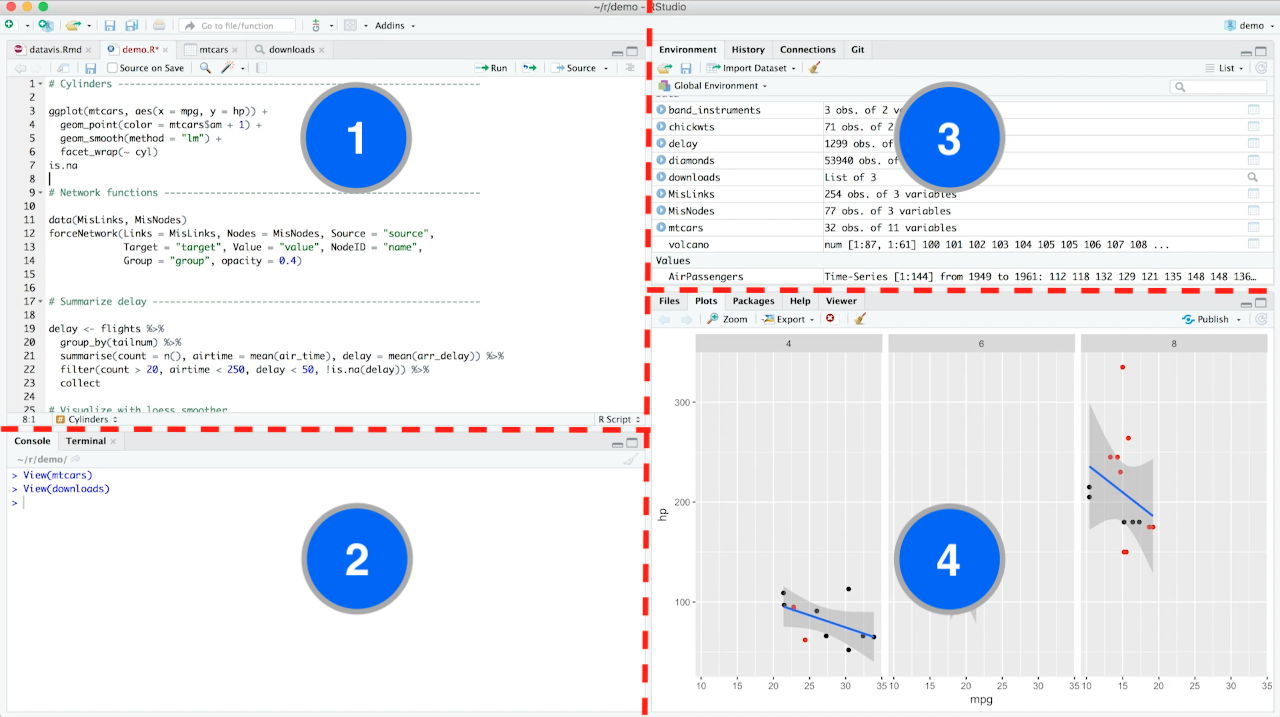
\includegraphics{images/introtods6.png}
\caption{Tampilan RStudio}
\end{figure}
\end{frame}

\begin{frame}{Membuat Proyek}
\protect\hypertarget{membuat-proyek}{}
\begin{columns}[T]
\begin{column}{0.5\textwidth}
Project merupakan sebuah folder seperti yang sudah sering kita buat. Di
R folder tersebut difungsikan untuk menyimpan segala sesuatu yang kita
buat di Rstudio secara otomatis kedalam folder tersebut. Keuntungan yang
didapatkan adalah kita memiliki fokus folder yang sedang menjadi tempat
kerja kita.

\begin{enumerate}
\tightlist
\item
  File
\item
  New Project
\item
  New Directory
\item
  New Project
\item
  Directory Name
\item
  Create Project
\end{enumerate}
\end{column}

\begin{column}{0.5\textwidth}
Kenapa?

Karena di R kita \textbf{hanya akan bisa mengolah data yang bisa diimpor
kedalam R} atau benar-benar eksis dalam lingkungan R.

\begin{figure}
\centering
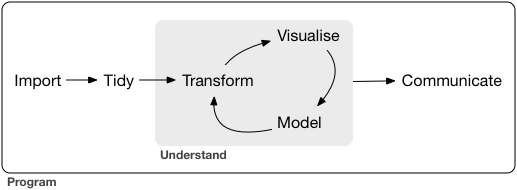
\includegraphics{images/introtods7.png}
\caption{Proses Pengolahan data di R}
\end{figure}
\end{column}
\end{columns}
\end{frame}

\begin{frame}[fragile]{Membuat dan menyimpan skrip/kumpulan perintah}
\protect\hypertarget{membuat-dan-menyimpan-skripkumpulan-perintah}{}
\begin{columns}[T]
\begin{column}{0.5\textwidth}
Skrip adalah kumpulan perintah yang kita buat untuk menyelesaikan atau
melakukan sesuatu dengan bahasa tertentu. Di R kita bisa membuat
beberapa skrip sesuai dengan peruntukannya.

\begin{enumerate}
\tightlist
\item
  R Scirpt \texttt{(.R)} umumnya digunakan untuk melakukan pengolahan
  data
\item
  R Markdown \texttt{(.Rmd)} umumnya digunakan untuk membuat laporan
\item
  Script-script lain yang biasa digunakan di pemerogaman seperti C, C++.
  CSS, dan lain sejennisnya
\end{enumerate}
\end{column}

\begin{column}{0.5\textwidth}
\begin{figure}
\centering
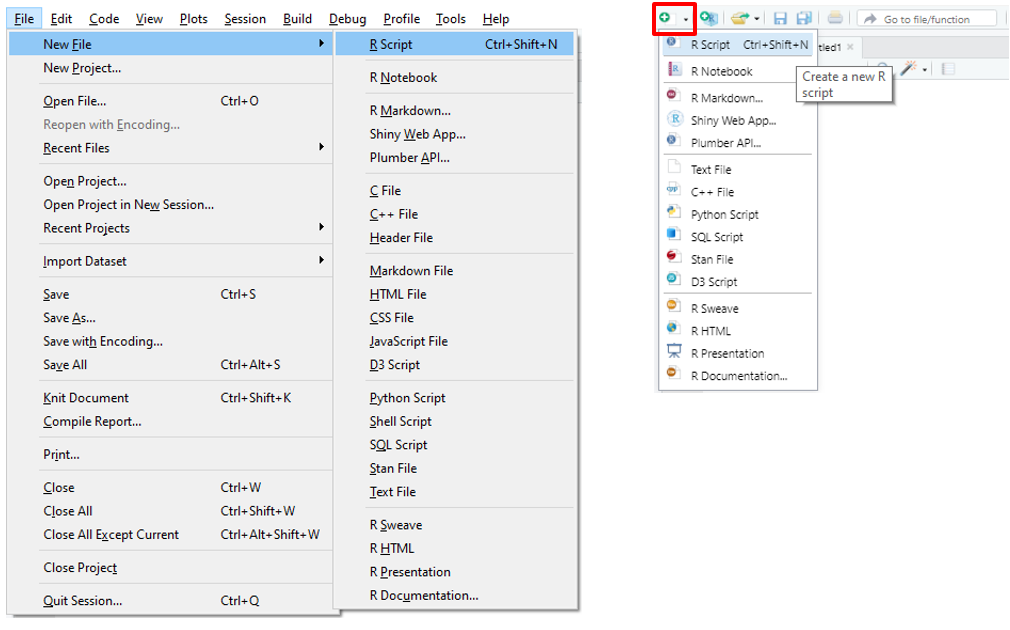
\includegraphics{images/introtods8.png}
\caption{Menu untuk membuat skrip di Rstudio}
\end{figure}
\end{column}
\end{columns}
\end{frame}

\begin{frame}[fragile]{Aturan menulis skrip}
\protect\hypertarget{aturan-menulis-skrip}{}
\begin{columns}[T]
\begin{column}{0.5\textwidth}
\textbf{UMUM}

\begin{enumerate}
\tightlist
\item
  Nama objek tidak boleh menggunakan spasi atau diawali dengan angka
  (\texttt{1namaobjek}, \texttt{nama\ objek})
\item
  Setiap perintah yang didahului dengan tanda pagar (\texttt{\#}) dibaca
  sebagai komentar
\item
  Komentar tidak akan dibaca sebagai perintah dan berfungsi untuk
  memberikan keterangan tambahan pada penulis atau yang menggunakan
  skrip
\item
  Objek di \texttt{R} bisa dibuat dengan menggunakan assigment. Misalnya
  \texttt{data1\ =\ 12\ *\ 19827} atau
  \texttt{data1\ \textless{}-12\ *\ 19827}
\end{enumerate}
\end{column}

\begin{column}{0.5\textwidth}
\textbf{Khusus}

\begin{figure}
\centering
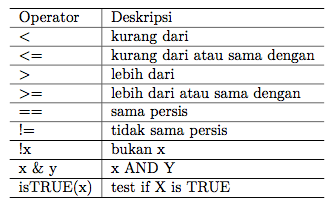
\includegraphics{images/introtods9.png}
\caption{Operator/tanda yang digunakan di R}
\end{figure}
\end{column}
\end{columns}
\end{frame}

\begin{frame}{Jenis skrip di Rstudio}
\protect\hypertarget{jenis-skrip-di-rstudio}{}
\begin{columns}[T]
\begin{column}{0.5\textwidth}
SKRIP R

\begin{figure}
\centering
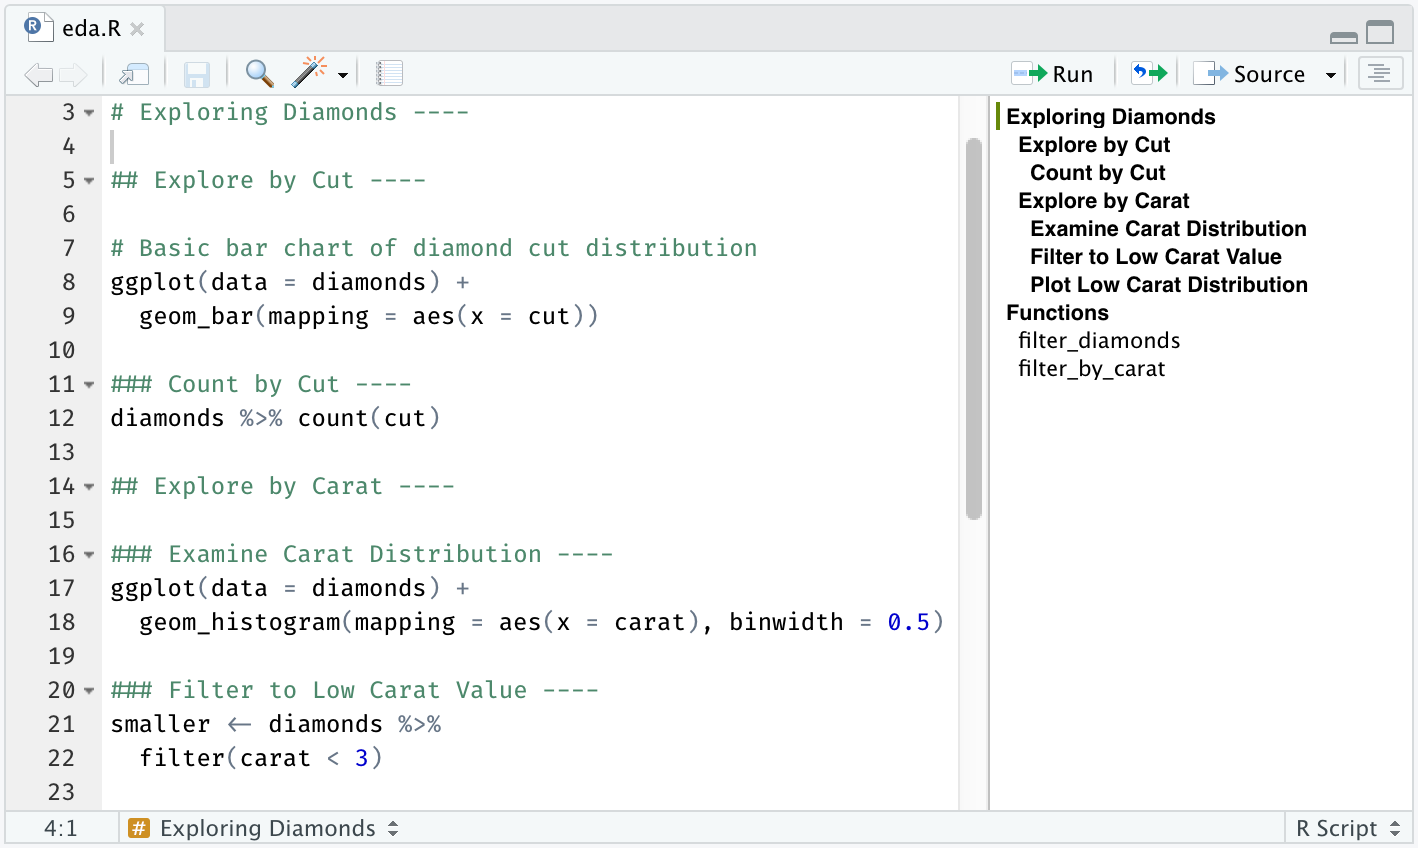
\includegraphics{images/introtods11.png}
\caption{Script R}
\end{figure}
\end{column}

\begin{column}{0.5\textwidth}
R MARKDOWN

\begin{figure}
\centering
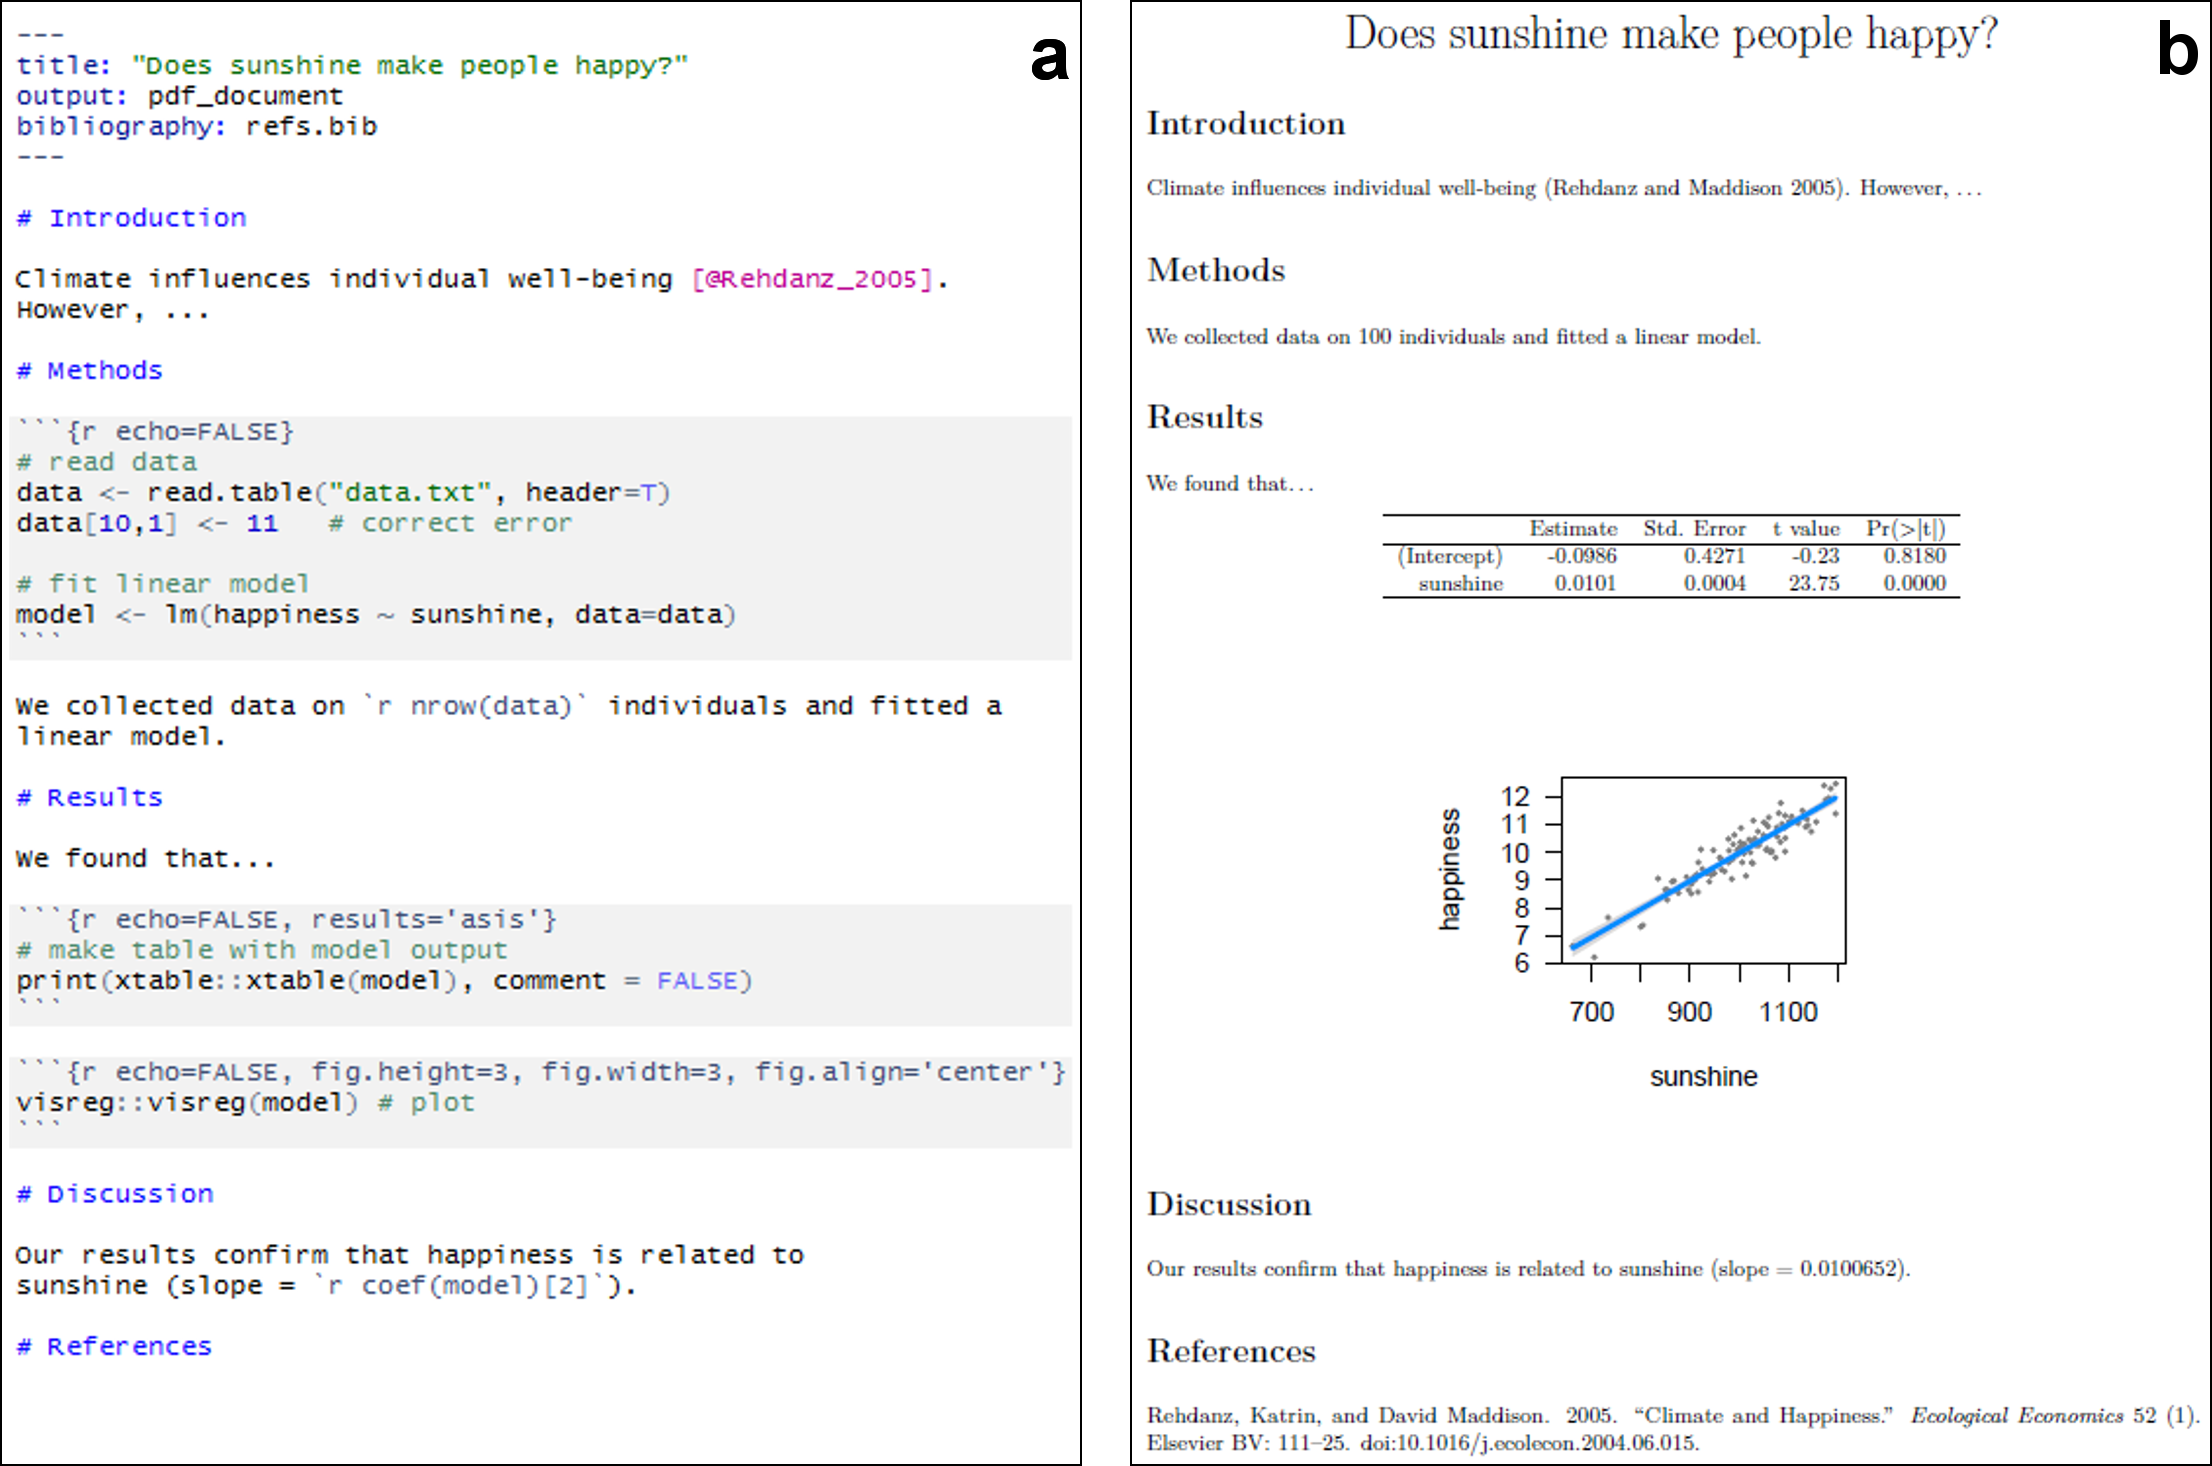
\includegraphics{images/introtods10.png}
\caption{R markdown}
\end{figure}
\end{column}
\end{columns}
\end{frame}

\hypertarget{library-dan-package}{%
\section{Library dan Package}\label{library-dan-package}}

\begin{frame}{Apa Library dan Package?}
\protect\hypertarget{apa-library-dan-package}{}
\begin{columns}[T]
\begin{column}{0.5\textwidth}
\begin{figure}
\centering

\includegraphics{images/introtods12.jpeg}
\caption{R markdown}
\end{figure}
\end{column}

\begin{column}{0.5\textwidth}
\begin{figure}
\centering
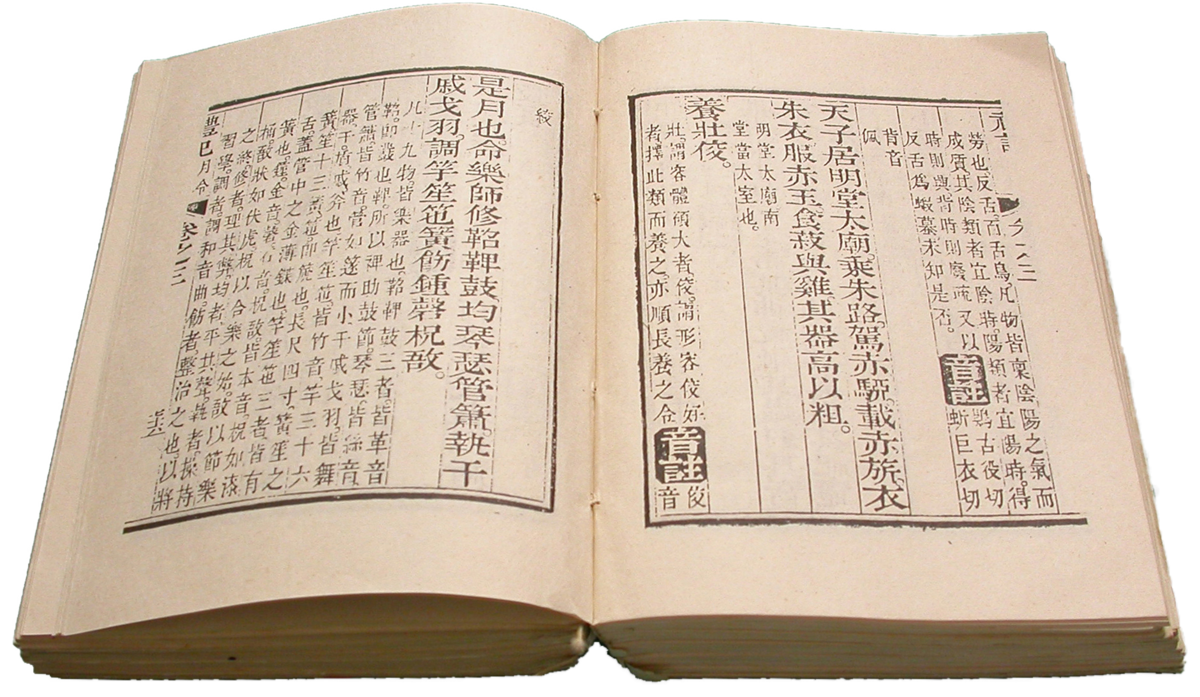
\includegraphics{images/introtods13.png}
\caption{R markdown}
\end{figure}
\end{column}
\end{columns}
\end{frame}

\begin{frame}[fragile]{Mendapatkan Library}
\protect\hypertarget{mendapatkan-library}{}
\begin{itemize}
\tightlist
\item
  Library atau package hanya perlu diinstall sekali
\item
  Library dan package perlu dipanggil kembali dalam setiap sesi baru R
\item
  Sebuah sesi baru di R dimulai dari saat membuka atau merstart R hingga
  menutup atau merestart kembali
\item
  Semua Library dan package dibuat secara terbuka (seperti wikipedia)
\item
  Library dan package dapat diinstall dengan menggunakan sintaks
  \texttt{install.packages(namaPackage)}
\item
  Library dan package sama-sama dipanggil menggunakan sintak
  \texttt{library()}
\item
  Semua Library dan package yang dikelola di kurasi oelh R dapat dilihat
  di: \url{https://cran.r-project.org/}
\end{itemize}
\end{frame}

\begin{frame}[fragile]{Menggunakan fungsi dalam package}
\protect\hypertarget{menggunakan-fungsi-dalam-package}{}
Fungsi dalam r terdiri dari nama\_fungsi(argumen1, argumen2, dst).
Bisanya dibuat dengan cara sebagai berikut.

\begin{Shaded}
\begin{Highlighting}[]
\CommentTok{\# pembuatan fungsi}
\NormalTok{fungsi\_modulo }\OtherTok{\textless{}{-}} \ControlFlowTok{function}\NormalTok{(argumen1)\{}
\NormalTok{  hasil }\OtherTok{=}\NormalTok{ argumen1}\SpecialCharTok{\%\%}\DecValTok{2}
  \FunctionTok{return}\NormalTok{(hasil)}
\NormalTok{\}}

\CommentTok{\# penggunaan fungsi}
\FunctionTok{fungsi\_modulo}\NormalTok{(}\AttributeTok{argumen1 =} \DecValTok{7}\NormalTok{)}
\end{Highlighting}
\end{Shaded}

Setiap fungsi dari dalam pacakge juga memiliki format seperti, sehingga
ketika kita akan menggunakannya kita perlu tahu terlebih dahulu argumen
yang dibutuhkannya.
\end{frame}

\begin{frame}[fragile]{Your Turn 1!}
\protect\hypertarget{your-turn-1}{}
\begin{enumerate}
\tightlist
\item
  Buatlah sebuah project di Rstudio!
\item
  Buatlah sebuah skrip \texttt{.R} di project yang telah dibuat!
\item
  Tulislah perintah untuk menginstall package \texttt{tidyverse},
  \texttt{tidytext}, dan \texttt{igraph}!
\end{enumerate}
\end{frame}

\hypertarget{fungsidasar}{%
\section{Fungsi-fungsi Dasar}\label{fungsidasar}}

\begin{frame}[fragile]{Fungsi paste}
\protect\hypertarget{fungsi-paste}{}
\begin{columns}[T]
\begin{column}{0.4\textwidth}
Terdapat dua fungsi paste, yaitu \texttt{paste()} dan \texttt{paste0()}.
Keduanya memiliki fungsi utama yang sama yaitu untuk meletakan sebuah
objek berdampingan dengan objek lainnya.

\begin{quote}
Mirip dengan fungsi paste yang mungkin telah sering kita gunakan saat
menggunakan komputer
\end{quote}
\end{column}

\begin{column}{0.6\textwidth}
Contoh:

\begin{Shaded}
\begin{Highlighting}[]
\NormalTok{teks1 }\OtherTok{\textless{}{-}} \StringTok{"aku adalah"}
\NormalTok{teks2 }\OtherTok{\textless{}{-}} \StringTok{"raja rimba"}

\NormalTok{teks12 }\OtherTok{\textless{}{-}} \FunctionTok{paste}\NormalTok{(teks1, teks2, }\AttributeTok{sep =} \StringTok{" "}\NormalTok{)}
\NormalTok{teks12}

\NormalTok{teks0 }\OtherTok{\textless{}{-}} \FunctionTok{paste0}\NormalTok{(teks1, teks2)}
\NormalTok{teks0}

\NormalTok{teks }\OtherTok{\textless{}{-}} \FunctionTok{paste0}\NormalTok{(teks1, }\StringTok{" "}\NormalTok{, teks2)}
\NormalTok{teks}
\end{Highlighting}
\end{Shaded}
\end{column}
\end{columns}
\end{frame}

\begin{frame}[fragile]{Fungsi if dan else}
\protect\hypertarget{fungsi-if-dan-else}{}
\begin{columns}[T]
\begin{column}{0.45\textwidth}
Fungsi ini digunakan untuk memilih output sesuai dengan kondisi yang
sudah ditentukan. Sering dinyatakan dengan
\texttt{JIKA\ ...\ MAKA\ ...}.

Kondisinya Nilai Tim A = 10, sementara Nilai Tim B = 8, skrip di R bisa
dibaca JIKA \texttt{nilai\ tim\ A\ lebih\ dari\ tim\ B} MAKA cetak
tulisan \texttt{TIM\ A\ adalah\ juaranya} jika tidak MAKA cetak
\texttt{TIM\ B\ adalah\ juaranya}
\end{column}

\begin{column}{0.55\textwidth}
Contoh:

\begin{Shaded}
\begin{Highlighting}[]
\NormalTok{Tim\_A }\OtherTok{=} \DecValTok{10}
\NormalTok{Tim\_B }\OtherTok{=} \DecValTok{8}

\ControlFlowTok{if}\NormalTok{ (Tim\_A }\SpecialCharTok{\textgreater{}}\NormalTok{ Tim\_B) \{}
  \FunctionTok{print}\NormalTok{(}\StringTok{"Tim A adalah juaranya"}\NormalTok{)}
\NormalTok{\} }\ControlFlowTok{else} \ControlFlowTok{if}\NormalTok{(Tim\_A }\SpecialCharTok{==}\NormalTok{ Tim\_B)\{}
  \FunctionTok{print}\NormalTok{(}\StringTok{"Seri"}\NormalTok{)}
\NormalTok{\} }\ControlFlowTok{else}\NormalTok{ \{}
  \FunctionTok{print}\NormalTok{(}\StringTok{"Tim B adalah juaranya"}\NormalTok{)}
\NormalTok{  \}}
\end{Highlighting}
\end{Shaded}
\end{column}
\end{columns}
\end{frame}

\begin{frame}[fragile]{Fungsi for-Loop}
\protect\hypertarget{fungsi-for-loop}{}
\begin{columns}[T]
\begin{column}{0.5\textwidth}
Fungsi \texttt{for-Loop} juga disebut perluangan. Digunakan untuk
melakukan hal-hal yang sama secara berulang sesuai dengan batas yang
ditentukan.

Fungsi ini akan terasa manfaatnya jika kita memiliki data yang cukup
banyak dan harus melakukan sebuah hal yang sama pada setiap observasi
yang dimiliki.
\end{column}

\begin{column}{0.5\textwidth}
Contoh:

\begin{Shaded}
\begin{Highlighting}[]
\ControlFlowTok{for}\NormalTok{ (value }\ControlFlowTok{in}\NormalTok{ vector)\{}
\NormalTok{  statements}
\NormalTok{\}}

\NormalTok{vektor }\OtherTok{\textless{}{-}} \FunctionTok{c}\NormalTok{(}\DecValTok{1}\SpecialCharTok{:}\DecValTok{5}\NormalTok{)}
\CommentTok{\# loop }
\ControlFlowTok{for}\NormalTok{(i }\ControlFlowTok{in}\NormalTok{ vektor)\{}
  \FunctionTok{print}\NormalTok{(i)}
\NormalTok{\}}
\end{Highlighting}
\end{Shaded}
\end{column}
\end{columns}
\end{frame}

\begin{frame}[fragile]{Fungsi-fungsi untuk melihat data (\texttt{str()},
\texttt{class()} dan \texttt{summary()})}
\protect\hypertarget{fungsi-fungsi-untuk-melihat-data-str-class-dan-summary}{}
\begin{columns}[T]
\begin{column}{0.5\textwidth}
Fungsi-fungsi di atas digunankan untuk melihat struktur, kelas, dan
rangkuman data. \texttt{str()} bisa dibaca struktur, \texttt{class()}
atau kelas digunakan untuk mengetahui jenis data yang ada dalam data,
apakah ia data frame, list, matrix atau lainnya. Sementara summary akan
lebih banyak digunakan saat melakukan eksplorasi data.
\end{column}

\begin{column}{0.5\textwidth}
\begin{Shaded}
\begin{Highlighting}[]
\FunctionTok{library}\NormalTok{(tidyverse)}

\NormalTok{df1 }\OtherTok{=}\NormalTok{ mtcars}

\FunctionTok{str}\NormalTok{(df1)}
\FunctionTok{class}\NormalTok{(df1)}
\FunctionTok{summary}\NormalTok{(df1)}
\end{Highlighting}
\end{Shaded}
\end{column}
\end{columns}
\end{frame}

\begin{frame}{Your Turn 2!}
\protect\hypertarget{your-turn-2}{}
\begin{enumerate}
\item
  Data A = 6 dan B = 187, jika A = genap, dan B = Ganjil, maka cetak
  ``Ganjil Genap'', jika A dan B genap, maka cetak ``Genap'', JIKA A dan
  B ganjil semua maka cetak Ganjil, JIKA A ganjil dan B genap, maka
  cetak ``Ganjil genap'', JIKA tidak memenuhi kondisi sebelumnya, maka
  cetak ``genap''.
\item
  A adalah sebuah distribusi angka antara 10 sampai dengan 1000 sebanyak
  100, buatlah fungsi loop dimana setiap menemukan angka genap console
  mencetak ``Genap'' sementara jika menemukan angka ganjil tidak
  mencetak apapun.
\end{enumerate}
\end{frame}

\hypertarget{dataType}{%
\section{Jenis-jenis data yang umum digunakan}\label{dataType}}

\begin{frame}[fragile]{Vectors}
\protect\hypertarget{vectors}{}
\begin{columns}[T]
\begin{column}{0.35\textwidth}
Vector merupakan sebuah tipe data gabungan yang berisi beberapa elemen
\texttt{atomic} berjenis sama. Untuk membuat sebuah vector, digunakan
perintah kombinasi \texttt{c()}.

Untuk mengakses vector bisa menggunakan tanda \texttt{namaVector{[}{]}}.
Misalnya, \texttt{a{[}1{]}}, berarti mengakses vektor ke-1 dari
\texttt{a}.
\end{column}

\begin{column}{0.65\textwidth}
Contoh:

\begin{Shaded}
\begin{Highlighting}[]
\NormalTok{a }\OtherTok{\textless{}{-}} \FunctionTok{c}\NormalTok{(}\DecValTok{1}\NormalTok{,}\DecValTok{2}\NormalTok{,}\FloatTok{5.3}\NormalTok{,}\DecValTok{6}\NormalTok{,}\SpecialCharTok{{-}}\DecValTok{2}\NormalTok{,}\DecValTok{4}\NormalTok{)}
\NormalTok{b }\OtherTok{\textless{}{-}} \FunctionTok{c}\NormalTok{(}\StringTok{"one"}\NormalTok{,}\StringTok{"two"}\NormalTok{,}\StringTok{"three"}\NormalTok{)}
\NormalTok{c }\OtherTok{\textless{}{-}} \FunctionTok{c}\NormalTok{(}\ConstantTok{TRUE}\NormalTok{,}\ConstantTok{TRUE}\NormalTok{,}\ConstantTok{FALSE}\NormalTok{,}\ConstantTok{TRUE}\NormalTok{,}\ConstantTok{FALSE}\NormalTok{)}
\end{Highlighting}
\end{Shaded}
\end{column}
\end{columns}
\end{frame}

\begin{frame}[fragile]{Data Frame}
\protect\hypertarget{data-frame}{}
\begin{columns}[T]
\begin{column}{0.5\textwidth}
Data frame juga disebut data flat atau rata, yaitu sebuah data yang
setiap barisnya memiliki kolom yang sama, dan setiap kolomnya memiliki
baris yang sama.

Untuk mengakses data frame bisa menggunaan tanda dollar \texttt{\$}.
Misalnya \texttt{datasiswa\$name}, berarti mengakses kolom \texttt{name}
dari data \texttt{datasiswa}. Sementara jika
\texttt{datasiswa\$name{[}3{]}}, berarti mengakses bari ke-3 dari kolom
\texttt{name} dalam \texttt{datasiswa}.
\end{column}

\begin{column}{0.5\textwidth}
Contoh:

\begin{Shaded}
\begin{Highlighting}[]
\NormalTok{id }\OtherTok{\textless{}{-}} \FunctionTok{c}\NormalTok{(}\DecValTok{1}\NormalTok{,}\DecValTok{2}\NormalTok{,}\DecValTok{3}\NormalTok{,}\DecValTok{4}\NormalTok{)}
\NormalTok{name }\OtherTok{\textless{}{-}} \FunctionTok{c}\NormalTok{(}\StringTok{"tom"}\NormalTok{, }\StringTok{"jerry"}\NormalTok{, }
          \StringTok{"dora"}\NormalTok{, }\StringTok{"emon"}\NormalTok{)}
\NormalTok{score }\OtherTok{\textless{}{-}} \FunctionTok{c}\NormalTok{(}\FloatTok{85.4}\NormalTok{,}\FloatTok{78.3}\NormalTok{,}
           \FloatTok{88.9}\NormalTok{,}\DecValTok{90}\NormalTok{) }

\CommentTok{\# membuat data frame dari kolom}
\NormalTok{datasiswa }\OtherTok{\textless{}{-}} \FunctionTok{data.frame}\NormalTok{(id,}
\NormalTok{                        name,}
\NormalTok{                        score)}
\end{Highlighting}
\end{Shaded}
\end{column}
\end{columns}
\end{frame}

\begin{frame}[fragile]{Lists}
\protect\hypertarget{lists}{}
\begin{columns}[T]
\begin{column}{0.5\textwidth}
List merupakan tipe data gabungan yang mirip dengan Vector, namun list
memungkinkan penggunaan elemen-elemen dengan tipe data dan jenis
variabel berbeda.

Untuk mengakses list kita bisa menggunakan
\texttt{namalist{[}{[}nama/indeks{]}{]}}. Misalnya
\texttt{all\_list{[}{[}1{]}{]}}, berarti mengakses list ke 1 dari
\texttt{all\_list}. Sementara jika untuk mengakses elemen spesifik dari
sebuah indeks dalam list kita bisa menggunakan skema
\texttt{namalist{[}{[}nama/indeks{]}{]}{[}indeks{]}} dan seterusnya.
\end{column}

\begin{column}{0.5\textwidth}
Contoh:

\begin{Shaded}
\begin{Highlighting}[]
\NormalTok{w }\OtherTok{\textless{}{-}} \FunctionTok{list}\NormalTok{(}\AttributeTok{name=}\StringTok{"Fred"}\NormalTok{, }
          \AttributeTok{age=}\DecValTok{25}\NormalTok{, }
          \AttributeTok{height=}\FloatTok{159.7}\NormalTok{)}
\NormalTok{x }\OtherTok{\textless{}{-}} \FunctionTok{list}\NormalTok{(}\StringTok{"saya"}\NormalTok{,}\FloatTok{5.4}\NormalTok{,}\DecValTok{1}\NormalTok{,}\ConstantTok{FALSE}\NormalTok{)}

\NormalTok{all\_list }\OtherTok{=} \FunctionTok{list}\NormalTok{(datasiswa, w, x)}
\end{Highlighting}
\end{Shaded}
\end{column}
\end{columns}
\end{frame}

\begin{frame}{Your Turn 3!}
\protect\hypertarget{your-turn-3}{}
\begin{enumerate}
\item
  Buatlah dua data frame. Data frame pertama memiliki 3 kolom dan 5
  baris dan beri nama df1, lalu buat data frame kedua, dengan 5 kolom
  dan 4 baris.
\item
  Buatlah list dengan nama list\_df dari dua data frame yang sudah
  dibuat.
\end{enumerate}
\end{frame}


\section[]{}
\frame{\small \frametitle{Table of Contents}
\tableofcontents}
\end{document}
